\documentclass[conference,letterpaper]{IEEEtran}
\usepackage{cite}
\usepackage{graphicx}
\usepackage{url}
\usepackage[hidelinks]{hyperref}

\graphicspath{{figures/}{waveforms/}}
\urlstyle{same}
\newcommand{\insn}[1]{\texttt{#1}}
\newcommand{\wave}[1]{\includegraphics[width=.93\linewidth]{#1}}

\begin{document}

\title{Design and Verification of a Single-Cycle RV32I Processor: Phase 1}
\author{\IEEEauthorblockN{Ankit Raj Singh, Rashmi Anand, Ayush, Saumya, and Samiksha Jangid}
\IEEEauthorblockA{Department of CSE (AI)\\Newton School of Technology, Sonipat}}
\maketitle

\begin{abstract}
This project implements a 32-bit single-cycle arithmetic processor in Verilog as the first phase of a ten-instruction RV32I design. The integrated datapath executes ADD, SUB, AND, OR, XOR, and ADDI. Load, store, and branch controls are checked at the module level. Five Icarus Verilog suites pass across 15 testbenches. The integrated test checks 14 instruction steps, and all 14 RTL modules pass Verilator lint and Yosys synthesis and structural checks. A waveform from the integrated test shows the ADD result and its register writeback edge.
\end{abstract}

\begin{IEEEkeywords}
RV32I, single-cycle processor, Verilog, datapath, RTL verification
\end{IEEEkeywords}

\section{Literature Review}
RV32I fixes the position of each register field wherever it appears and uses instruction bit 31 as the sign bit for the immediates used here \cite{rv32i}. The Phase~1 core therefore wires the register indices directly from the instruction and uses one block to assemble and sign-extend I-, S-, and B-type immediates.

In the textbook single-cycle datapath, instruction fetch, operand selection, ALU execution, and any register writeback fit within one clock period \cite{cod,ddca}. Phase~1 adopts that organization for arithmetic, separates instruction decoding from ALU operation selection, and tests the memory and branch paths at the module level before integrating them.

\section{Proposed Solution}
\subsection{Scope and Datapath}
Phase~1 connects instruction fetch, decode, operands, execution, and register writeback (Fig.~\ref{fig:datapath}). The byte-addressed program counter (PC) resets synchronously to zero and increments by four during sequential fetch. The instruction store reads combinationally and returns the canonical \insn{ADDI x0,x0,0} for invalid or uninitialized locations. The register file exposes two asynchronous read ports and one rising-edge write port. Reads of \insn{x0} produce zero and writes to it are discarded.

\begin{figure}[!t]
\centering
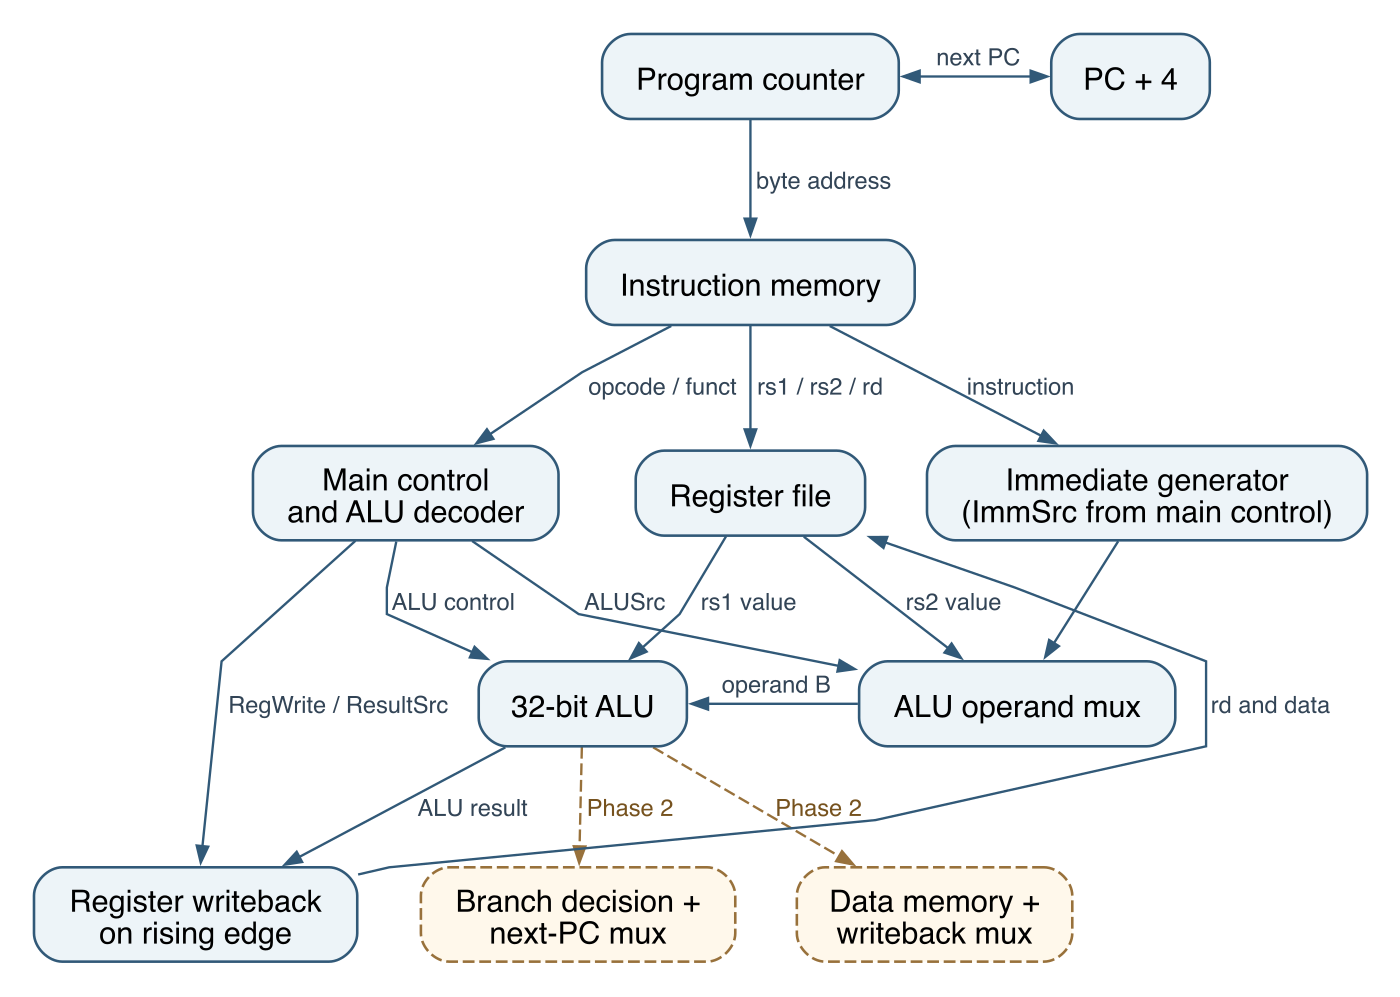
\includegraphics[width=\columnwidth]{phase1-datapath.png}
\caption{Phase~1 arithmetic datapath. Dashed boxes show the planned memory and branch integration points.}
\label{fig:datapath}
\end{figure}

\begin{figure*}[!t]
\centering
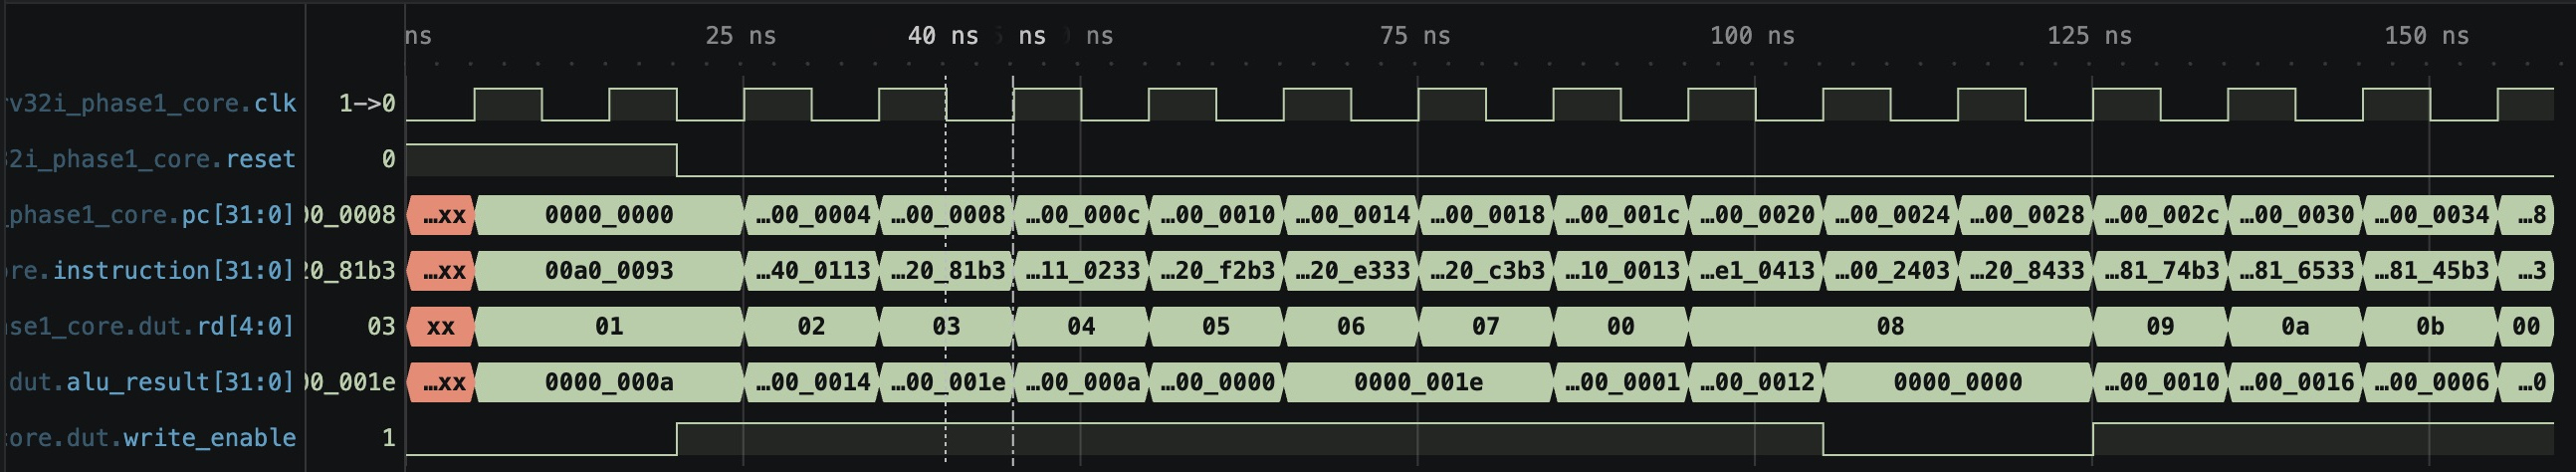
\includegraphics[width=\linewidth]{tb_rv32i_phase1_core.jpg}
\caption{ADD and writeback in the integrated Phase~1 test. The markers identify the ADD inputs at 40~ns and the rising clock edge at 45~ns. The image is a direct capture of a VCD opened in VaporView, cropped to the viewer.}
\label{fig:add}
\end{figure*}

\subsection{Instruction Decode}
The main decoder checks the opcode and \insn{funct3}. For register-register instructions it checks the full \insn{funct7} field. \insn{ALUSrc} selects the second register operand or the sign-extended immediate. \insn{ALUOp} directs the ALU decoder to select addition, subtraction, or an R-type operation. Unsupported encodings deassert register writes and memory or branch requests. Table~\ref{tab:control} summarizes the control outputs.

\begin{table}[!t]
\caption{Main Decoder Control Outputs}
\label{tab:control}
\centering
\begin{tabular}{@{}lccc@{}}
\hline
Instruction(s) & Control bits$^{a}$ & \insn{ALUOp} & \insn{ImmSrc} \\
\hline
ADD, SUB, AND, OR, XOR & \insn{100000} & \insn{10} & \insn{11} \\
ADDI                    & \insn{110000} & \insn{00} & \insn{00} \\
LW                      & \insn{111010} & \insn{00} & \insn{00} \\
SW                      & \insn{010100} & \insn{00} & \insn{01} \\
BEQ, BNE                & \insn{000001} & \insn{01} & \insn{10} \\
Unsupported             & \insn{000000} & \insn{11} & \insn{11} \\
\hline
\end{tabular}

\smallskip
\parbox{\columnwidth}{\footnotesize $^{a}$ In order: \insn{RegWrite}, \insn{ALUSrc}, \insn{MemRead}, \insn{MemWrite}, \insn{ResultSrc}, \insn{Branch}.}
\end{table}

\subsection{State Updates and Phase Boundary}
The core writes an ALU result on a rising edge when reset is low, \insn{RegWrite} is high, and \insn{ResultSrc} selects the ALU. The six arithmetic and logic instructions exercise this path end to end. The decoder generates the expected controls for \insn{LW}, \insn{SW}, \insn{BEQ}, and \insn{BNE}, and the standalone tests exercise storage and branch-path components. Phase~2 connects data memory writeback and conditional next-PC selection for those four instructions.

\section{Verification and Results}
Icarus Verilog~13.0 ran the fetch, storage, ALU, operand-selection, and Phase~1 integration suites \cite{icarus}. All 15 testbenches passed. The 20-vector control test compared the control bits, ALU operation, and immediate for supported and unsupported encodings. The integrated test covered 14 instruction steps, including writes to \insn{x0}, a negative immediate, and suppressing writeback for a decoded load. The one-word memory test checked in-range and out-of-range behavior. All 14 RTL modules passed Verilator~5.054 lint \cite{verilator} and Yosys synthesis and structural checks \cite{yosys}.

Table~\ref{tab:results} lists the first seven demo instructions. The VaporView capture in Fig.~\ref{fig:add} shows the ADD at 40~ns with PC \insn{0x08}, destination \insn{x3}, ALU result \insn{0x1E}, and write enable high. The rising edge at 45~ns commits the value as the PC advances to SUB. The testbench confirms \insn{x3 = 30} after the edge. The appendix includes the remaining 14 VCD screenshots. The repository provides the test runners and full-resolution captures. The course lectures and labs provide the background for the project \cite{mcalectures,mcalabs}.

\begin{table}[!t]
\caption{Verified Arithmetic Register Writeback}
\label{tab:results}
\centering
\begin{tabular}{@{}llr@{}}
\hline
PC & Instruction & Result (decimal) \\
\hline
\insn{0x00} & \insn{addi x1,x0,10} & \insn{x1 = 10} \\
\insn{0x04} & \insn{addi x2,x0,20} & \insn{x2 = 20} \\
\insn{0x08} & \insn{add x3,x1,x2}  & \insn{x3 = 30} \\
\insn{0x0C} & \insn{sub x4,x2,x1}  & \insn{x4 = 10} \\
\insn{0x10} & \insn{and x5,x1,x2}  & \insn{x5 = 0} \\
\insn{0x14} & \insn{or x6,x1,x2}   & \insn{x6 = 30} \\
\insn{0x18} & \insn{xor x7,x1,x2}  & \insn{x7 = 30} \\
\hline
\end{tabular}
\end{table}

\section{Individual Contributions}
\textbf{Ankit Raj Singh} implemented the program counter, instruction memory, and sequential fetch path and verified each block and the integrated fetch sequence.

\textbf{Rashmi Anand} implemented the register file and data memory and verified their read, write, and address behavior with the storage tests.

\textbf{Ayush} implemented the ALU and ALU decoder and verified arithmetic, logic, and operation selection.

\textbf{Saumya} implemented the immediate generator, three multiplexers, and branch target calculator. She verified sign extension and the selectors for ALU operand B, writeback data, and the next PC.

\textbf{Samiksha Jangid} implemented the main decoder and integrated the arithmetic core. She added decoder and core tests, a test runner, memory-depth regression coverage, and submission documentation.

\section{Conclusion}
Phase~1 verifies six arithmetic and logic instructions from fetch through writeback. The standalone tests verify storage and branch-path behavior for Phase~2 integration.

\appendix[Waveform Evidence]
Figures~\ref{fig:fetch}--\ref{fig:decode} show VCDs from revision \insn{21ec7a2}, captured in VaporView~1.6.1 and cropped to the viewer. The repository lists the five commands to regenerate these traces.

\begin{figure*}[!p]
\centering
\wave{tb_program_counter.jpg}\par\smallskip
\wave{tb_instruction_memory.jpg}\par\smallskip
\wave{tb_rv32i_core.jpg}
\caption{Fetch tests, from top to bottom. The program counter follows the supplied next address and resets to zero. The instruction memory returns the canonical NOP for invalid or uninitialized locations. The integrated fetch test checks sequential PC and instruction values.}
\label{fig:fetch}
\end{figure*}

\begin{figure*}[!p]
\centering
\wave{tb_register_file.jpg}\par\smallskip
\wave{tb_data_memory.jpg}\par\smallskip
\wave{tb_memory_depth_one.jpg}
\caption{Storage tests, from top to bottom. The register file commits a write to \insn{x6} on a rising edge. The data memory stores and reads \insn{0x19} at byte address \insn{0x40}. The final test checks access and bounds for depth-one memories.}
\label{fig:storage}
\end{figure*}

\begin{figure*}[!p]
\centering
\wave{tb_alu.jpg}\par\smallskip
\wave{tb_alu_control.jpg}
\caption{ALU tests. The first trace shows the result and zero flag for arithmetic and logic operations. The second shows the decoder output for supported operations and code 7 for unsupported combinations.}
\label{fig:alu}
\end{figure*}

\begin{figure*}[!p]
\centering
\wave{tb_immediate_generator.jpg}\par\smallskip
\wave{tb_alu_src_mux.jpg}\par\smallskip
\wave{tb_writeback_mux.jpg}
\caption{Immediate and data selection tests, from top to bottom. The immediate generator sign-extends I-, S-, and B-fields. \insn{ALUSrc} switches operand B between a register value and the immediate. \insn{ResultSrc} selects ALU or memory data for writeback.}
\label{fig:mux}
\end{figure*}

\begin{figure*}[!p]
\centering
\wave{tb_next_pc_mux.jpg}\par\smallskip
\wave{tb_branch_target.jpg}
\caption{Standalone next-PC and branch target tests. \insn{PCSrc} selects PC+4 or the branch target. The target calculator adds a signed branch offset to the current PC.}
\label{fig:branch}
\end{figure*}

\begin{figure*}[!p]
\centering
\wave{tb_control_unit.jpg}
\caption{Main decoder test for arithmetic and separate load, store, and branch controls. Unsupported encodings leave the state-changing controls inactive.}
\label{fig:decode}
\end{figure*}

\begin{thebibliography}{8}
\bibitem{rv32i} A. Waterman and K. Asanovi\'c, Eds., \emph{The RISC-V Instruction Set Manual, Volume I: Unprivileged ISA}, ver. 20191213. RISC-V Foundation, Dec. 2019, ch. 2. [Online]. Available: \href{https://docs.riscv.org/reference/isa/v20191213/_attachments/riscv-unprivileged.pdf}{RISC-V specification archive}
\bibitem{cod} D. A. Patterson and J. L. Hennessy, \emph{Computer Organization and Design RISC-V Edition: The Hardware/Software Interface}, 2nd ed. Morgan Kaufmann, 2020, ch. 4.
\bibitem{ddca} S. L. Harris and D. M. Harris, \emph{Digital Design and Computer Architecture: RISC-V Edition}. Morgan Kaufmann, 2021, ch. 7.
\bibitem{icarus} S. Williams, \emph{Icarus Verilog}, ver. 13.0. [Online]. Available: \href{https://github.com/steveicarus/iverilog/releases/tag/v13_0}{Release notes}
\bibitem{verilator} W. Snyder, \emph{Verilator}, ver. 5.054. [Online]. Available: \href{https://verilator.org/guide/latest/changes.html#verilator-5-054-2026-11-01}{Release notes}
\bibitem{yosys} C. Wolf, \emph{Yosys Open SYnthesis Suite}. [Online]. Available: \href{https://yosyshq.net/yosys/documentation.html}{Documentation}
\bibitem{mcalectures} \textquotedblleft{}Modern Computer Architecture lectures.\textquotedblright{} Course lectures.
\bibitem{mcalabs} \textquotedblleft{}Modern Computer Architecture labs.\textquotedblright{} Course laboratory materials.
\end{thebibliography}

\end{document}
